\section{Validation and Evaluation} \label{sec:chp2-sec7}
This section first discusses different methods of validation and then presents different measurements of validation. 
\subsection{Validation}
Validation, or cross-validation, is an important part of the classification framework that ensures its generalization.
Validation also avoids having a bias classifier or overfitting. 
\acf{kcv} and \acf{loocv} are two different techniques for performing validation. 
In this section, we first discuss different methods for validation of a data classification framework and then present various measurements of its evaluation. 

\acl{kcv} randomly divides the dataset into $k$ partitions of equal size.
Among the $k$ partitions, one is used as the test set, and the classifier is trained on the remaining $k-1$ subsets. 
Using \ac{kcv}, the classification is performed $k$ times to ensure that each of the subsets is used as the test set once.

Leave-one-out-cross-validation can be seen as a form of \ac{kcv} when $k = n$, n is the total number of samples.
In this validation, the classification is repeated $n$ rounds. 
At each round, one sample is left out for testing and the classifier is trained on the remaining samples.
This method is suitable when dealing with a small or unbalanced dataset.    

\subsection{Evaluation}
Evaluation is another important part of the framework that measures the quality and performance of the framework.
While solving classification problems, a simple way to quantify the performance of the classifier is to look at the confusion matrix.
The confusion matrix is an error table that shows the performance of the algorithm.
Each row of the matrix represents instances in the predicted class and each column shows instances in their actual class (or vice-versa). 
Figure~\ref{fig:CM} shows the table and graphical representation of a confusion matrix.

\colorlet{circle edge}{blue!50}
\colorlet{circle area}{blue!20}


% Definition of circles
% \def\myRadius{1.5cm}
% \def\vennSpace{(0,0) rectangle (6cm,4cm)}
% \def\predictedCircle{(2cm,2cm) circle (\myRadius)}
% \def\actualCircle{(4cm,2cm) circle (\myRadius)}
% \def\myLabelRadius{1.3cm}

\def\myRadius{.75cm}
\def\vennSpace{(0,0) rectangle (3cm,2cm)}
\def\predictedCircle{(1cm,1cm) circle (\myRadius)}
\def\actualCircle{(2cm,1cm) circle (\myRadius)}
\def\myLabelRadius{.60cm}

\tikzset{fillbase/.style={fill=circle area, draw=circle edge, thick},
         filled/.style={pattern=crosshatch dots, draw=circle edge, thick},
         outline/.style={draw=circle edge, thick}}

\def\drawPredicted{
    \draw[outline] \predictedCircle node (x){}; % {$\bullet$};
    \node [above left=\myLabelRadius of x, anchor=center, outer sep=0](p){$P$};
    \node  at (p.300) {$+$};
    \node  at (p.120) {$-$};
}

\def\drawActual{
    \draw[outline] \actualCircle node (x){}; % {$\bullet$};
    \node [above right=\myLabelRadius of x, anchor=center, outer sep=0](a){$A$};
    \node  at (a.60) {$-$};
    \node  at (a.240) {$+$};
}

% Define the different metrics: tp, tn, fp, fn
\def\tp{
      \draw[outline] \vennSpace;
      \begin{scope}
        \clip \predictedCircle;
        \fill[filled] \actualCircle;
      \end{scope}
      \drawPredicted
      \drawActual
      % \draw[outline] (current bounding box.south west)
      %   rectangle (current bounding box.north east);
}

\def\tn{
      \draw[outline] \vennSpace;
  \begin{scope}[even odd rule]
    \fill[filled] \vennSpace
      \actualCircle
      \predictedCircle;
    \clip \actualCircle;
    \fill[white] \predictedCircle;
  \end{scope}
  \drawPredicted
  \drawActual
}

\def\fp{
      \draw[outline] \vennSpace;
      \begin{scope}
        \clip \predictedCircle;
        \fill[filled, even odd rule]
              \predictedCircle \actualCircle;
      \end{scope}
      \draw[outline] \vennSpace;
      \drawPredicted
      \drawActual
}

\def\fn{
      \draw[outline] \vennSpace;
      \begin{scope}
        \clip \actualCircle;
        \fill[filled, even odd rule]
              \actualCircle \predictedCircle;
      \end{scope}
      \draw[outline] \vennSpace;
      \drawPredicted
      \drawActual
}

\def\se{
  \fill[fillbase] \actualCircle;
      \begin{scope}
        \clip \predictedCircle;
        \fill[filled] \actualCircle;
      \end{scope}
      \draw[outline] \vennSpace;
      \drawPredicted
      \drawActual
}


\def\sp{
  \fill[fillbase, even odd rule]
    \vennSpace \actualCircle;
  \begin{scope}[even odd rule]
    \fill[filled] \vennSpace
      \actualCircle
      \predictedCircle;
    \clip \actualCircle;
    \fill[white] \predictedCircle;
  \end{scope}
  \draw[outline] \vennSpace;
  \drawPredicted
  \drawActual
  }


\begin{figure}[t]
  \def\myRadius{.65cm}
  \def\vennSpace{(0,0) rectangle (2.6cm,1.6cm)}
  \def\predictedCircle{(.8cm,.8cm) circle (\myRadius)}
  \def\actualCircle{(1.8cm,.8cm) circle (\myRadius)}
  \def\myLabelRadius{.450cm}
\centering{
\subfloat[]{
%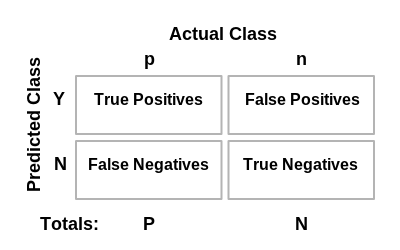
\includegraphics[scale= 0.3]{Chapter2/Figures/confusion-matrix_1.png}}\hfill
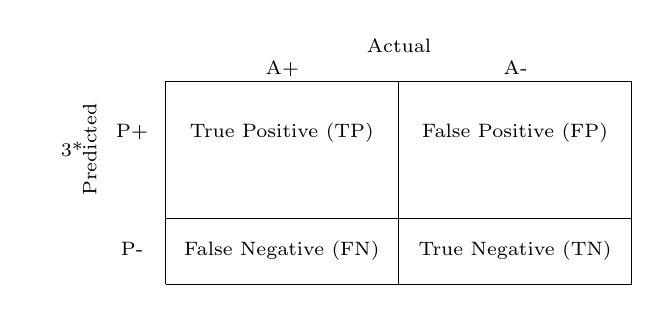
\begin{tikzpicture}[scale=0.4]
      \node at (0,0){
      \scriptsize{
        \begin{tabular}{
            >{\centering}m{1em} >{\centering}m{1em} >{\centering}m{1in} >{\centering\arraybackslash}m{1in}}
          % c>{\centering}m{2em}ccc}
          & & \multicolumn{2}{c}{ Actual}\\
          & & A+ & A- \\
          \cline{3-4}
          & \multicolumn{1}{c|}{} & \multicolumn{1}{c|}{} & \multicolumn{1}{c|}{}\\
          \multirow{3}{*}{\rotatebox[origin=c]{90}{Predicted}}& \multicolumn{1}{c|}{P+} &  \multicolumn{1}{c|}{True Positive (TP)} & \multicolumn{1}{c|}{False Positive (FP)} \\
          &\multicolumn{1}{c|}{}  & \multicolumn{1}{c|}{}& \multicolumn{1}{c|}{} \\
          \cline{3-4}
          & \multicolumn{1}{c|}{} &\multicolumn{1}{c|}{} & \multicolumn{1}{c|}{}\\
          
          & \multicolumn{1}{c|}{P-} &\multicolumn{1}{c|}{False Negative (FN)}  &\multicolumn{1}{c|}{True Negative (TN)}\\
          & \multicolumn{1}{c|}{} &\multicolumn{1}{c|}{} & \multicolumn{1}{c|}{}\\
          \cline{3-4}
          \end{tabular}
      }};
    \end{tikzpicture}
    }\\

  \subfloat[]{
    \label{fig:evaluation-confusion_matrix}
    \begin{tikzpicture}[scale=0.4]
      \node at (0,0){
        \begin{tabular}{
            >{\centering}m{1em} >{\centering}m{1em} >{\centering}m{1in} >{\centering\arraybackslash}m{1in}}
          % c>{\centering}m{2em}ccc}
          & & \multicolumn{2}{c}{ Actual Class }\\
          & & A+ & A- \\
          % \parbox[t]{2mm}{\multirow{2}{*}{\rotatebox[origin=c]{90}{\usebox \centering Predicted Class}}}& P+ &  \tikz{\tp} & \tikz{\fp} \\
          \multirow{3}{*}{\rotatebox[origin=c]{90}{Predicted Class}}& P+ &  \tikz{\tp} & \tikz{\fp} \\
          & P- & \tikz{\fn} & \tikz{\tn}
        \end{tabular}
      };
    \end{tikzpicture}
  }
  }
  \caption[Confusion matrix]{Tabular (a) and graphical (b) representations of a confusion matrix with true and false positive samples (\acs{tp}, \acs{fp}) in the first row and false and true negative samples (\acs{fn}, \acs{tn}) in the second row (from left to right).}
  \label{fig:CM}
\end{figure}
True positive (\ac{tp}) and \acf{tn} instances are simply the samples that are correctly predicted to belong to the positive or negative class, respectively.
False positive (\ac{fp}) samples are predicted as the positive class while in reality they belong to the negative class; and \acf{fn} instances are predicted as the negative class while belonging to the positive class.
Various statistic measures are derived form the confusion matrix, among which the most popular ones are \acf{acc}, \acf{se}, \acf{sp}, and precision.

Accuracy (see Eq.~\ref{eq:acc}) measures the overall performance of the algorithm by considering the number of instances classified correctly without considering their classes.
Although this measure is important, it can be misleading in real-world classification problems because an overfitted or biased classifier can have high accuracy while not performing as desired.
\begin{equation}
\ac{acc} = \frac{TP+TN}{TP+TN+FP+FN}~.
\label{eq:acc}
\end{equation} 
The sensitivity, recall or true positive rate is another statistic that measures an performance of the algorithm with respect to the positive class only.
\begin{equation}
\ac{se}	 = \frac{TP}{TP+FN}~.
\label{eq:se}
\end{equation}
Opposite to \ac{se}, \acl{sp} or true negative rate measures the algorithm's performance with respect to the negative class:
\begin{equation}
\acs{sp} = \frac{TN}{TN+FP}.
\label{eq:sp}
\end{equation}
Figure~\ref{fig:sesp} shows a graphical illustration of \ac{se} and \ac{sp} in the confusion matrix.
\begin{figure}
 \def\myRadius{.65cm}
 \def\vennSpace{(0,0) rectangle (2.6cm,1.6cm)}
 \def\predictedCircle{(.8cm,.8cm) circle (\myRadius)}
 \def\actualCircle{(1.8cm,.8cm) circle (\myRadius)}
 \def\myLabelRadius{.450cm}
  
\centering
\begin{tikzpicture}[scale=0.5]
      \def\seEquation{$SE = \frac{TP}{TP+FN}$}
      \def\spEquation{$SP = \frac{TN}{TN+FP}$}
      \node[label={[]below:\seEquation}](se){\tikz{\se}};
      \node[right=5pt of se, label={[]below:\spEquation}]{\tikz{\sp}};
      %\node[label={[]right:\seEquation}](se){\tikz{\se}};
      %\node[below=5pt of se, label={[]right:\spEquation}]{\tikz{\sp}};
\end{tikzpicture}
    
\caption[Sensitivity and Specificity]{Sensitivity and \acl{sp} evaluation, corresponding to the ratio of the doted area over the blue area.}
\label{fig:sesp}
\end{figure}

Precision or positive predictive value (PPV), as its name suggests, is a measure of the algorithms precision.
Considering an algorithm that is more biased towards the positive class, this algorithm has high \ac{se}, however, it is less precise, since it considers most of the instances as more or less positive.
\begin{equation}
precision = \frac{TP}{TP+FP}~.
\label{eq:ppv}
\end{equation} 

All the aforementioned measures can be used to quantify the performance of an algorithm.
They can also be combined to generate a graphical plot such as \acf{roc} or precision-recall curve.
The \ac{roc}~\cite{zweig1993receiver} is a graphical curve of \ac{se} against a \acf{fpr} or (1 - \ac{sp}).
The curve is constructed by varying the discriminant threshold of the classifier.
Adjusting the threshold will lead to classifying more \ac{tp} samples, usually at the cost of increasing \ac{fp}s.
Due to this property, the \ac{roc} is a valuable tool, specially in the medical field when having high \ac{se} is important.
%This tool allows us to analyze the cost of having the highest \ac{se} in the trade off \ac{fp}.
This tool allows us to analyze the cost of having the highest \ac{se} against the number of \ac{fp}.
This curve is shown in Fig.~\ref{fig:roccurve}.
Here each point represents an \ac{se}/\ac{sp} pair corresponding to the discriminant threshold.
The \ac{roc} curve statistics are often represented by the \acf{auc}, which is a single number corresponding to the area under the \ac{roc} curve.
The \ac{auc} varies between 0.5 to 1 for algorithms with an average to perfect performance.

\begin{figure}
\begin{center}
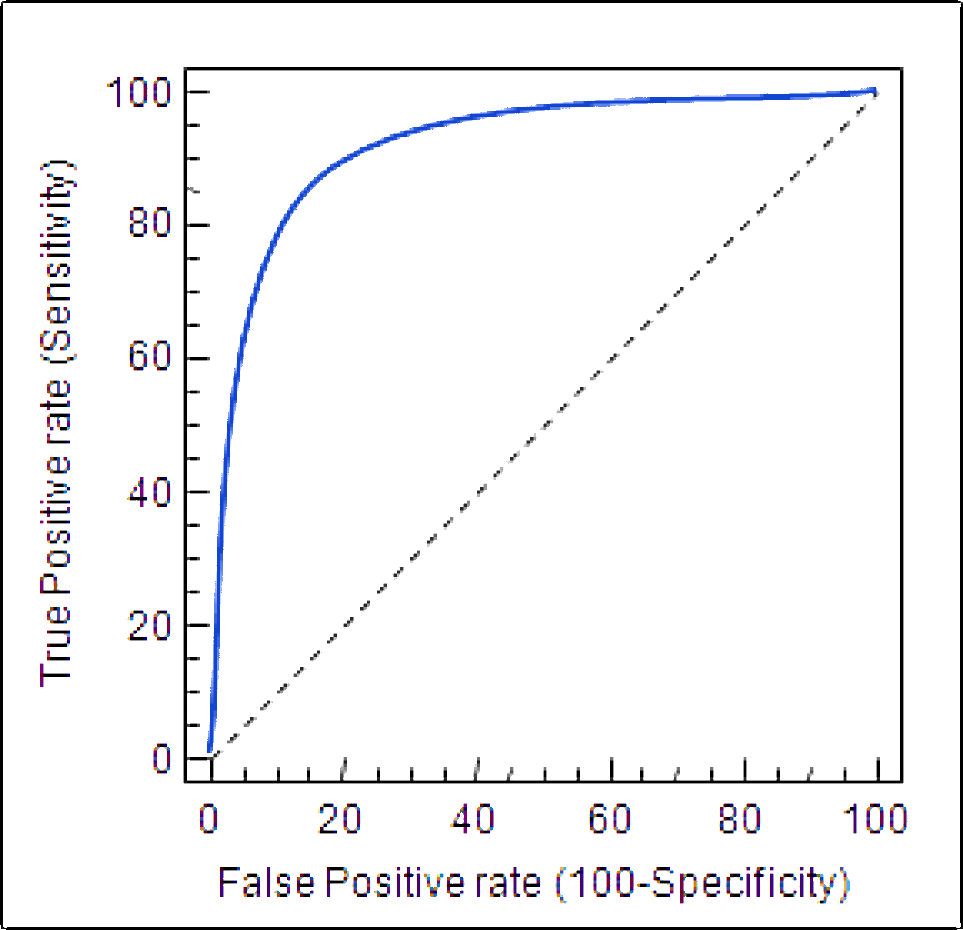
\includegraphics[scale=1]{Chapter2/Figures/roccurve2}
\end{center}
\caption[\ac{roc} curve]{\ac{roc} curve.}
\label{fig:roccurve}
\end{figure}



%%% Local Variables: 
%%% mode: latex
%%% TeX-master: "../thesis"
%%% End: 
